\chapter{\xlabel{pol2_image}POL-2 Image Display}
\label{sec:display}

\section{\xlabel{gaia}GAIA}

The \starlink\ package \gaia\ can be used to inspect the results of the data reduction. 
To plot the output vector catalogue onto the final non-polarized intensity map
first open up the I map in gaia:

\begin{terminalv}
% gaia iext.sdf
\end{terminalv}


Then In the main Gaia window, select the drop-down menu option Image Analysis / 
Polarimetry toolbox…. This should launch a new toolbox window entitled 
GAIA: Polarimetry. From this window, use the drop-down menu option 
File / Open to load the file mycat.FIT. This should then populate the lower part of the 
window with the contents of this polarimetry catalogue file. 
Each of the vectors in this file will be automatically overlaid on the main image window 
(see figure \ref{fig:gaia-plot-vectors1}).

\begin{figure}[t!]
\begin{center}
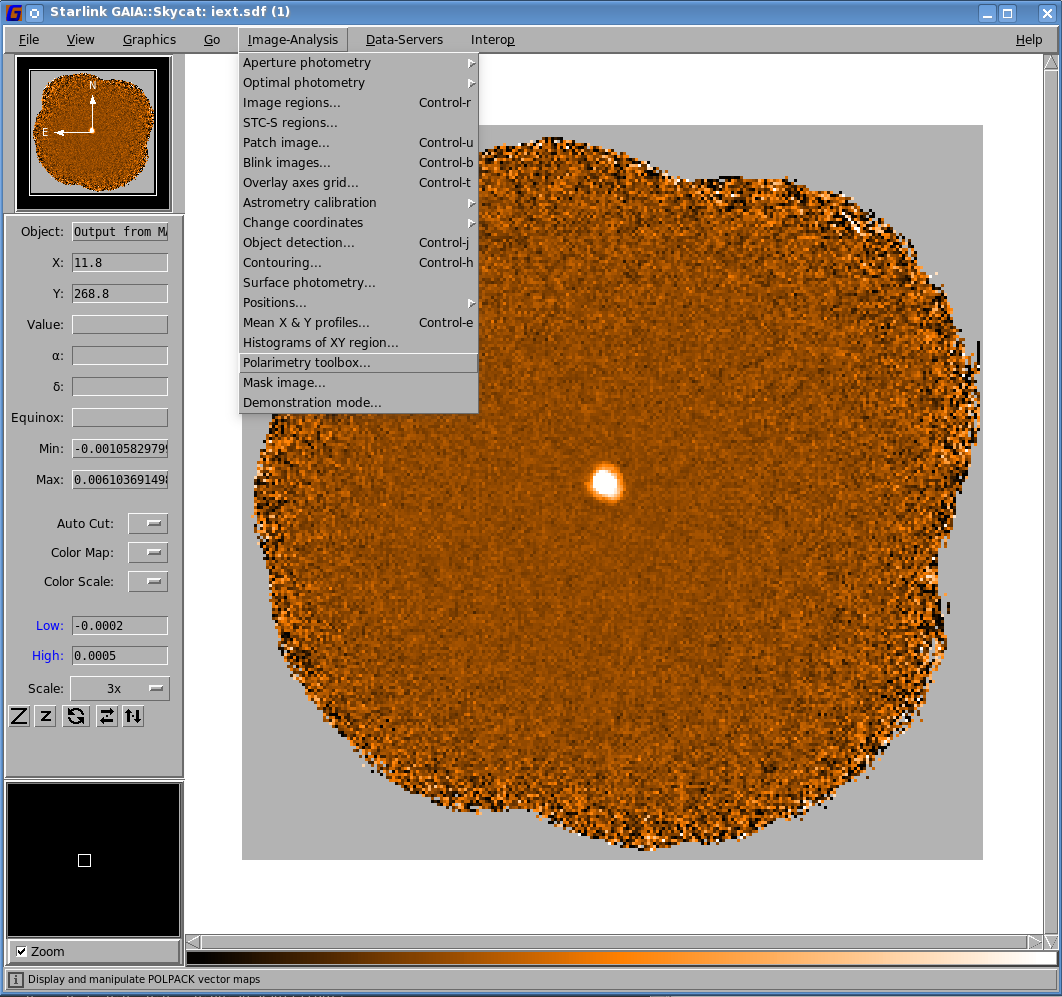
\includegraphics[width=0.46\linewidth]{sc22-gaia-plot-vectors-1.png}
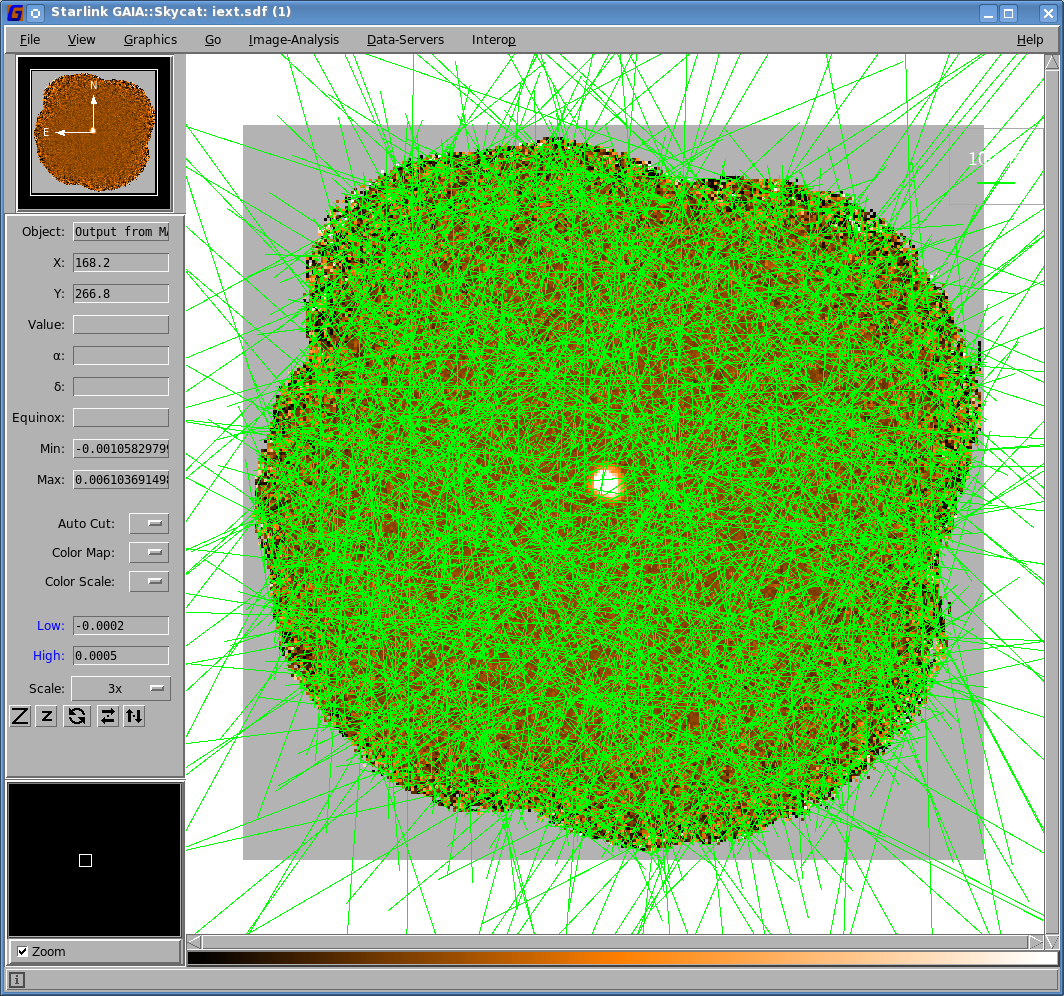
\includegraphics[width=0.46\linewidth]{sc22-gaia-plot-vectors-3.png}
\label{fig:gaia-plot-vectors1}
\caption [Over Plotting Vectors in GAIA]{
  \small Left: Opening up the polarimetry tool box in GAIA. Right: The initial POL-2 
vectors overplotted in GAIA.
}
\end{center}
\end{figure}

In order to filter the number of overlaid vectors down to a more useful number and size,
various options in the GAIA: Polarimetry window can be used. First, select the Rendering
tab on the left hand side. This will reveal a panel that will indicate which quantities 
are currently being used for the vector overlays. In this case, the Vector length is taken 
from the P column of the table, and the Vector angles are taken from the ANG column.

Currently the figure has too many vectors to be scientifically meaningful. To filter 
out most of the extraneous vectors, click on the Selecting tab, and set the Expression 
field to be the following:

\begin{terminalv}
$I/$DI>10
\end{terminalv}

\emph{Ensure you press return after entering in the above expression}.

The above expression selects the data points in the polarimetry table which have an 
associated non-polarized intensity (column I) more than 10 times greater than the 
associated error value for that intensity (column DI). To remove all of the other 
extraneous overlaid vectors, click on the Invert selection button in the GAIA: Polarimetry 
window, and then use the drop-down menu option Edit / Cut. This should leave just a 
small number of vectors clustering around the target object. 

\begin{figure}[t!]
\begin{center}
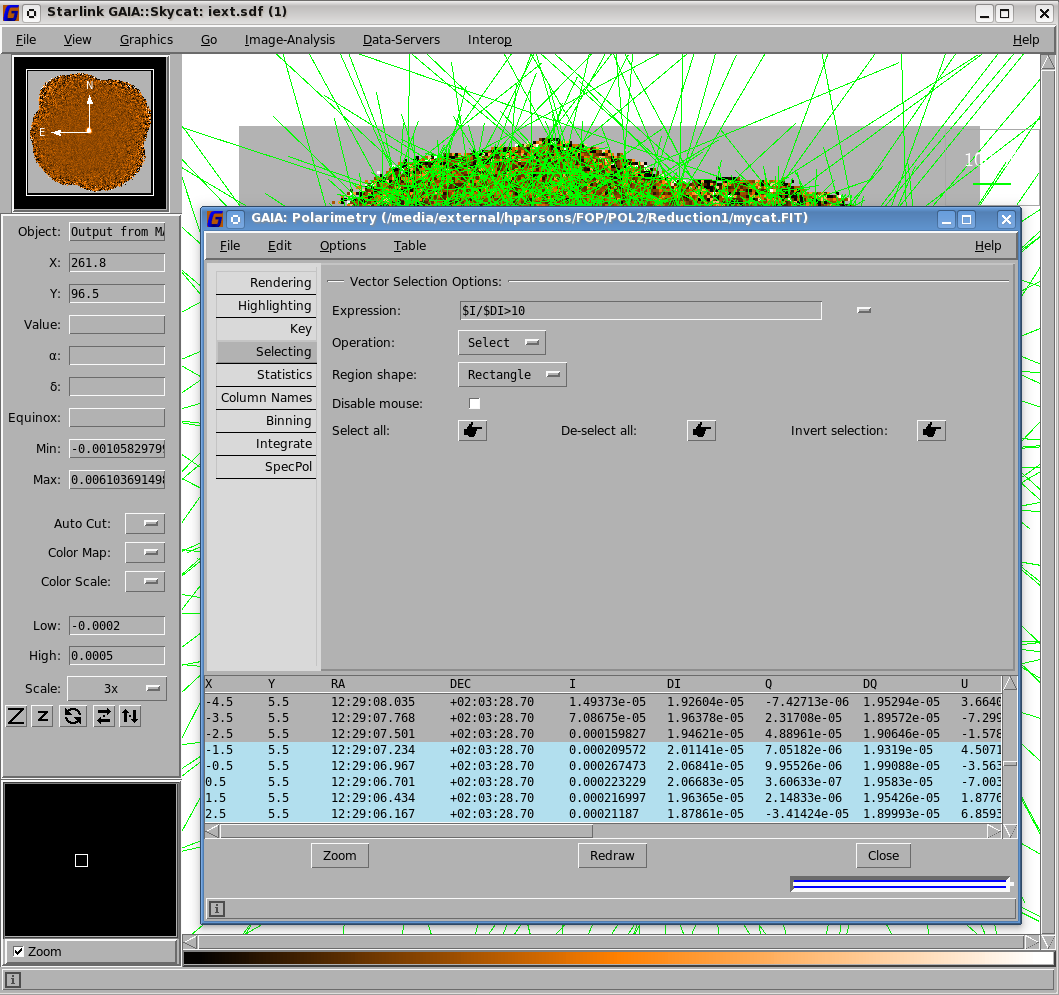
\includegraphics[width=0.46\linewidth]{sc22-gaia-plot-vectors-4.png}
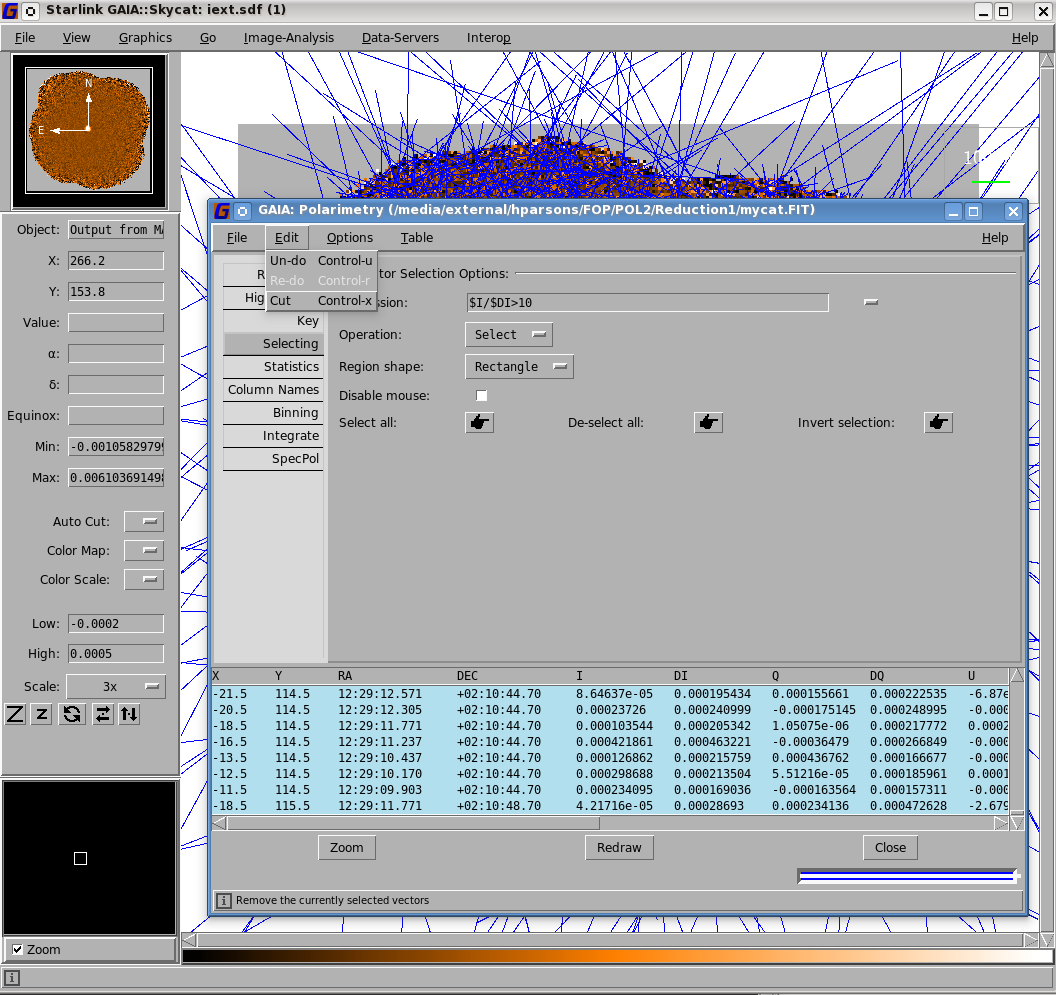
\includegraphics[width=0.46\linewidth]{sc22-gaia-plot-vectors-6.png}
\label{fig:gaia-plot-vectors2}
\caption [Selecting Vectors in GAIA]{
  \small Left: specifying vectors to display via the expression \$I/\$DI$>$10. This will only plot
vectors with an 850 micron intensity signal-to-noise ratio grater than 10 in GAIA. To ensure this is selected
ensure you press the carriage return after entering the expression. 
}
\end{center}
\end{figure}

Zooming in on the central region of the map, it can already be seen that the level of vector ordering 
(and hence polarization) is quite low (see figure \ref{fig:gaia-plot-vectors3}). If needed it is 
possible to change the scaling by selecting the Rendering tab in the GAIA: Polarimetry 
window, and increasing the vector scale.


\begin{figure}[t!]
\begin{center}
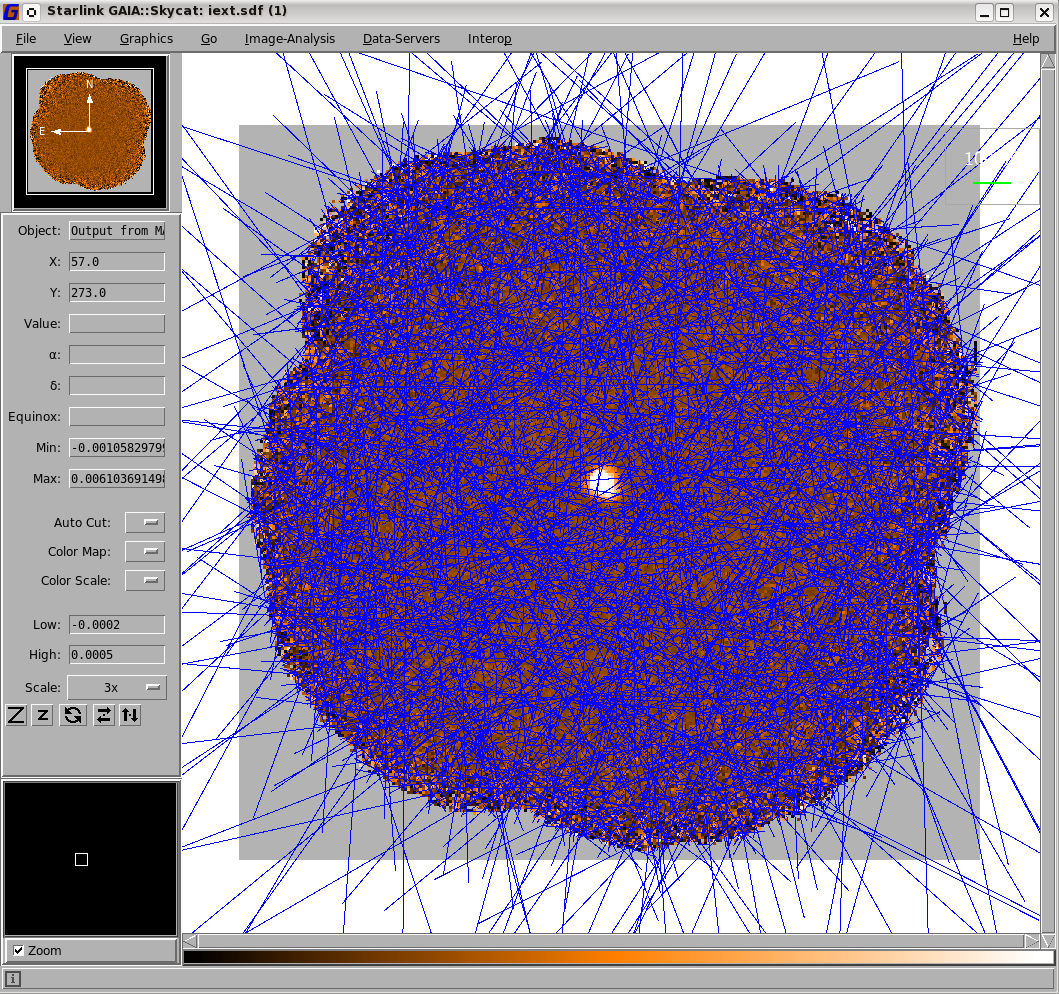
\includegraphics[width=0.44\linewidth]{sc22-gaia-plot-vectors-5.png}
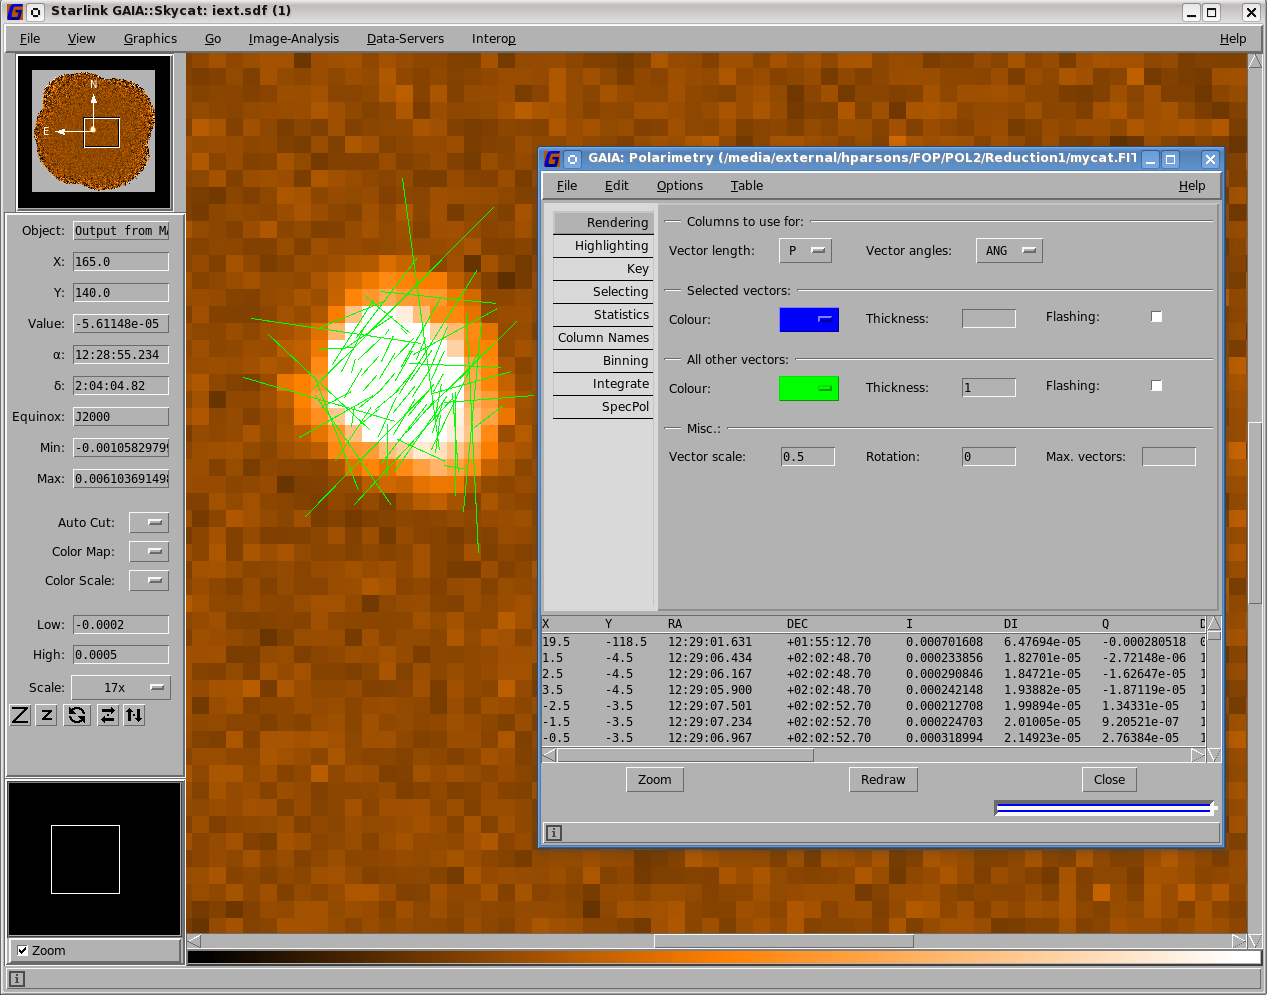
\includegraphics[width=0.52\linewidth]{sc22-gaia-plot-vectors-7.png}
\label{fig:gaia-plot-vectors3}
\caption [Over Plotting Vectors in GAIA]{
  \small Left: Selected vectors are marked in blue in this example, Right: after removal of selected
vectors all that remains are the vectors on the regions where \$I/\$DI$>$10. 
}
\end{center}
\end{figure}


\section{\xlabel{kappa}kappa}


